\documentclass[a4paper]{article}
\usepackage[utf8]{inputenc}
\usepackage[T1]{fontenc}
\usepackage{textcomp}
\usepackage{amsmath, amssymb, amsthm}
\usepackage{geometry}
\usepackage{tikz-cd}
\usepackage{mdframed}
\usepackage{microtype}
\usepackage{hyperref}
\usepackage{cleveref}

\usepackage[backend = biber, style = alphabetic]{biblatex}
\addbibresource{../references.bib}

% figure support
\usepackage{import}
\usepackage{xifthen}
\usepackage[textsize=tiny,colorinlistoftodos,obeyDraft]{todonotes}
\newcommand{\question}[1]{\todo[color=green!40]{#1}}
\usepackage{pdfpages}
\usepackage{transparent}
\newcommand{\incfig}[1]{%
	\def\svgwidth{\columnwidth}
	\import{./figures/}{#1.pdf_tex}
}

\pdfsuppresswarningpagegroup=1


\newcommand{\N}{\mathbb{N}}
\newcommand{\Z}{\mathbb{Z}}
\newcommand{\Q}{\mathbb{Q}}
\newcommand{\C}{\mathbb{C}}
\newcommand{\R}{\mathbb{R}}
\newcommand{\F}{\mathbb{F}}
\newcommand{\pro}{\mathbb{P}}
\newcommand{\aff}{\mathbb{A}}
\newcommand{\ltr}{\par \noindent \framebox[1\width]{ $\implies$ } \hspace{.2cm}}
\newcommand{\rtl}{\par \noindent \framebox[1\width]{ $\impliedby$ } \hspace{.2cm} }

\DeclareMathOperator{\coker}{coker}
\DeclareMathOperator{\id}{Id}
\DeclareMathOperator{\im}{Im}
\DeclareMathOperator{\spec}{Spec}
\DeclareMathOperator{\maxspec}{MaxSpec}
\DeclareMathOperator{\spf}{Spf}
\DeclareMathOperator{\proj}{Proj}
\DeclareMathOperator{\red}{red}
\DeclareMathOperator{\trop}{trop}
\DeclareMathOperator{\trdeg}{TrDeg}
\DeclareMathOperator{\divisor}{Div}
\DeclareMathOperator{\cov}{Cov}

\newcommand{\into}{\hookrightarrow}
\newcommand{\onto}{\twoheadrightarrow}
\newcommand{\divides}{\mid}
\newcommand{\notdivides}{\nmid}
\newcommand{\Gan}{\ensuremath{\mathbb{G} _m ^{\mathrm{an}}}}
\newcommand{\an}{{}^{\text{an}}}
\newcommand{\cox}{\widehat{\otimes}}

\newcommand{\st}{%
  \nonscript\;
  \ifnum\currentgrouptype=16
    \,\middle|\,
  \else
    \,|\,
  \fi
  \nonscript\;}

\theoremstyle{definition}
\newtheorem{definition}{Definition}[subsection]
\newtheorem{remark}[definition]{Remark}
\newtheorem{theorem}[definition]{Theorem}
\newtheorem{example}[definition]{Example}
\newtheorem{lemma}[definition]{Lemma}
\newtheorem{claim}[definition]{Claim}
\newtheorem{proposition}[definition]{Proposition}
\newtheorem{exercise}[definition]{Exercise}
\newtheorem{corollary}[definition]{Corollary}


\author{Micha\"el Maex}

\title{Berkovich geometry and models of curves}
\begin{document}
\maketitle	

\setcounter{section}{-1}
\section{Notation and conventions} \label{sec:notation_and_conventions}
Throughout the talk $K$ will be a field with a non-trivial, complete, non-archimedean norm. 
The main examples for this are (finite extensions of) $\Q_p, \C((t)), \F_q((t))$. 
Often we require $K$ to be either discretely valued, i.e. $|K^{\times }|$ is discrete. 
Sometimes we require $K$ to be algebraically closed. 

\begin{notation}
	\begin{align*}
		R &= \{a \in K \st |a| \le 1\}  \\
		\mathfrak{m}  &=  \{a \in K \st |a| < 1\} \\
		k &= \frac{R}{\mathfrak{m} }
	.\end{align*}
\end{notation}
The ring $R$ is always a local ring with unique maximal ideal $\mathfrak{m} $, and a DVR if  $K$ is discretely valued. We let $\pi$ be a uniformiser of $K$.  
As a scheme $\spec R$ consists of 2 points, the generic point with residue field $K$ and a closed point with residue field $k$. 

All norms we consider will be non-archimedean, i.e.\ they satisfy the stronger triangle inequality $|x + y| \le \max(|x|, |y|)$. 
I will freely switch between real valuations and norms, which are related by an exponentian relation.
\begin{align*}
	|x| = e^{-v(x)}, \quad v(x) = -\ln(|x|)
.\end{align*}

A curve will be a projective smooth connected 1-dimensional  variety over $K$. 

\section{Motivation for Berkovich Geometry} \label{sec:motivation_for_berkovich_geometry}

What makes algebraic geometry over $\C$ different from algebraic geometry over other fields is that there is an analytification functor that turn $\C$-varieties into $\C$-analytic spaces, i.e.\ complex manifolds that may have singularities. 
If we restrict this functor to the category of proper  $\C$-varieties, this functor is even fully faithful. This fact and a collection of results that act as a dictionary between the algebraic and analytic world are collectively known as the GAGA principles. 
They lead to an interesting interplay between complex analysis and algebraic geometry, which gives rise to topics like Hodge theory. 

A analysis is not limited to $\C$. In fact the only thing we need to work out a theory of analysis is a normed field, preferably a complete normed field. 
If this field is not $\C$ or $\R$ then it has to be either trivially valued or non-archimedean. \todo{find a citation for this}
The best known examples of these are the $p$-adic rationals $\Q_p$. 
There is in fact an entire theory of $p$-adic analysis. 

Varieties over $p$-adic fields and rings lay at the heart of arithmetic geometry. 
So it is a natural question to ask whether $p$-adic varieties, or more generally varieties over complete non-archimedean fields can be ``analytified'' in a suitable way, giving us an interplay between algebraic geometry and analysis that has been very fruitful in complex geometry. 

The first question that needs to be resolved, is what such an analytic space might be.
Over $\C$ we already had a theory of complex manifolds.
But if we try to construct $p$-adic manifolds, we quickly run into a problem.
The topology of $\Q_p$ or any non-archimedean field, is totally disconnected. 
This means that $p$-adic manifolds are very non-rigid and in particular the principle of analytic continuation fails. 
We will use $K$ to mean any complete non-archimedean field. Think $K = \Q_p$ or $K = \C((t))$. 

In 1960\todo{source} Tate was was the first one propose a solution. 
His idea was to still work with $p$-adic manifolds, but replace the topology, by $G$-topology. 
This is somewhat like an ordinary topology, but not al set theoretic covers of opens are topological covers. 
The topological covers are called admissible.
This works, but it hides a lot of the topology of the space in set of covers, which is difficult to grasp.

In 1990 Berkovich proposed his theory of $K$-analytic spaces - often called Berkovich spaces - which solves the disconnectedness problem by adding extra points to the space, which connect the disconnected components. 
The resulting space actually is a very nice topological space - hausdorff, locally compact, path-connected, \ldots - which is in stark contrast to the topology of $K$ itself.  

\begin{figure}[H]
    \centering
    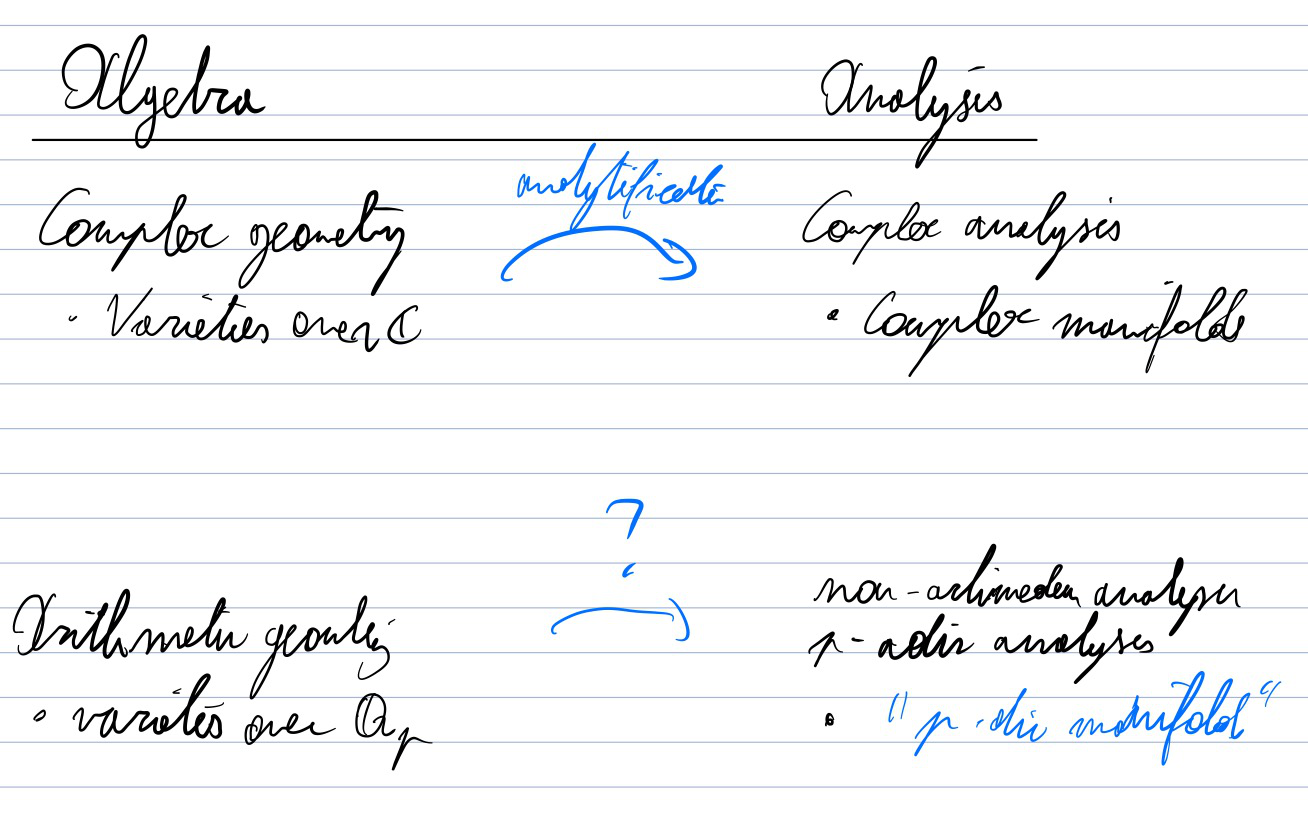
\includegraphics[width = .7\textwidth]{figures/analytification-comparison.png}
    \caption{analytification comparison}
    \label{fig:analytification-comparison}
\end{figure}

\begin{figure}[H]
    \centering
    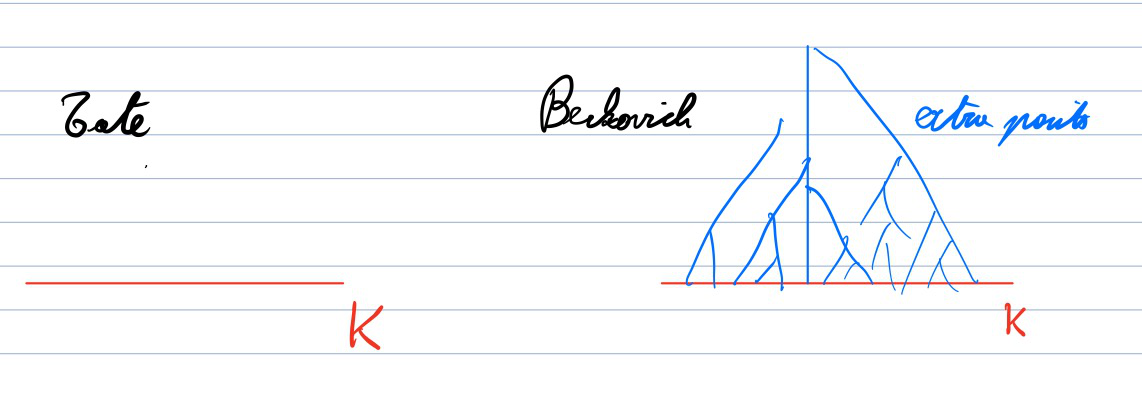
\includegraphics[width = .9\textwidth]{figures/affine-line-according-to-tate-and-berkovich.png}
    \caption{affine line according to tate and berkovich}
    \label{fig:affine-line-according-to-tate-and-berkovich}
\end{figure}
\section{Recap on non-archimedean (semi)-norms} \label{sec:recap_for_norms}



\begin{definition}
	Let $A$ be a ring. 
	A \emph{seminorm} on $A$ is a function  $|\cdot |: R \to [0, \infty)$ such that 
	\begin{enumerate}
		\item $|0| = 0, |1| = 1$ 
		\item $|x + y| \le \max(|x|, |y|) $ (strong triangle inequality)
		\item $|x\cdot y| \le |x| \cdot |y|$
	\end{enumerate}
	We can strengthen some of these axioms. 
	A seminorm is \emph{multiplicative} if $|x\cdot y| = |x|\cdot |y|$.
\end{definition}
All norms we encounter today are multiplicative. 
\begin{definition}
	If $f: (B, |\cdot |_B) \to A$ is a ring morphism and $B$ is a normed ring, then a seminorm $|\cdot |_A$ on $A$ extends the norm on $B$ if $|b|_B = |f(b)|_A, \forall b \in B$. 
\end{definition}

Norms are valuations are the same thing
\begin{definition}
	The \emph{kernel} of a norm $|\cdot |$ is $\ker |\cdot | =\{a \in A \st |a| = 0\} $. 
\end{definition}
\begin{proposition}
	The kernel of a norm $|\cdot |$ on $A$ is an ideal of $A$. 
	If $|\cdot |$ is multiplicative then $\ker |\cdot | $ is a prime ideal. 

\end{proposition}
\begin{proof}
	Suppose $a, b \in \ker |\cdot |, c \in A$. 
	Then $|a + b| \le \max(|a|, |b|) = 0$. So  $a + b \in \ker |\cdot |$. 
	Also $|c\cdot a| \le |c| \cdot |a| =0$. So $c\cdot A \in\ker|\cdot |$. 

	Suppose that $|\cdot |$ is multiplicative and $a\cdot b \in \ker|\cdot |$.
	Then $|a|\cdot |b| = |a\cdot b| =0$ so either $|a| = 0$ or $|b| = 0$. 
\end{proof}
The kernel of a multiplicative norm is a prime ideal in $R$. 
Note that every seminorm on field is necessarily a norm. 


\section{What is a Berkovich Space} \label{sec:what_is_a_berkovich_space}
\begin{definition}
	Let $A$ be a $K$-algebra, then the \emph{Berkovich spectrum of $A$} 
	is \[
		\mathcal{M} (A) =  \{\text{multiplicative seminorms on }A \text{ that extend the norm on } K\}  
	.\] 
\end{definition}
This comes with a natural projection $i: \mathcal{M} (A) \to \spec A : |\cdot |_x \mapsto \ker |\cdot |_x$. 
Given a point $y \in \spec A$, a seminorm on $A$ with kernel $y$ is the same as a norm on $A / y$, which is the same as a norm on $Q(A/ y) = \kappa(y)$. 
So instead of giving a seminorm $|\cdot |_x$ on $A$ we may instead give a pair $(y, |\cdot |_x')$ with $y = \ker|\cdot |_x \in \spec R$ and $|\cdot |_x'$ a norm on  $v$. 
\[
	|\cdot |_A \text{ with }\ker = x \quad \cong \quad (x, |\cdot |_{A / x}) \quad \cong \quad (x, |\cdot |_{\kappa(x)})
.\] 

This allows us to globalize the definition to general schemes. 
\begin{definition}\label{def:berkovich_analytification_explicit}
	The \emph{Berkovich analitification} of $K$-scheme, as a set is \[
		X\an = \{(x, |\cdot |)  \mid x\in X, |\cdot | \text{ a norm on } \kappa(x) \text{ extending the norm on }K \} 
	.\] 
	This comes equipped with a canonical projection map $i: X\an \to X, (x, |\cdot |) \mapsto  x$.
	
	$X\an $ comes with a topology which we define to be the coarsest topology such that 
	\begin{itemize}
		\item $i: X\an \to X$ is continuous, i.e. $X\an$ is a finer space than  $X$. 
		\item For every open $U \subset X$ and $f \in \mathcal{O}_X(U)$ the map  \[
				|f|: i^{-1}(U) \to \R^{+}: (x, |\cdot |) \mapsto  |f(x)|
		\] 
		is continuous.
	\end{itemize}
\end{definition}
We usually only define this for $K$-varieties, and so will we in this talk. 

\subsection{What do these Berkovich spaces look like?} \label{sec:what_do_these_berkovich_spaces_look_like?}

Suppose that $x \in X$ is a closed point, then $\kappa(x)$ is a finite extension of $K$.
It a non-obvious theorem that there is a unique extension of the norm on $K$ to $\kappa(x)$, whence $i^{-1}(x)$ is a single point.
So in particular we may embed $X_{cl} \into X\an$.  

\begin{figure}[H]
    \centering
    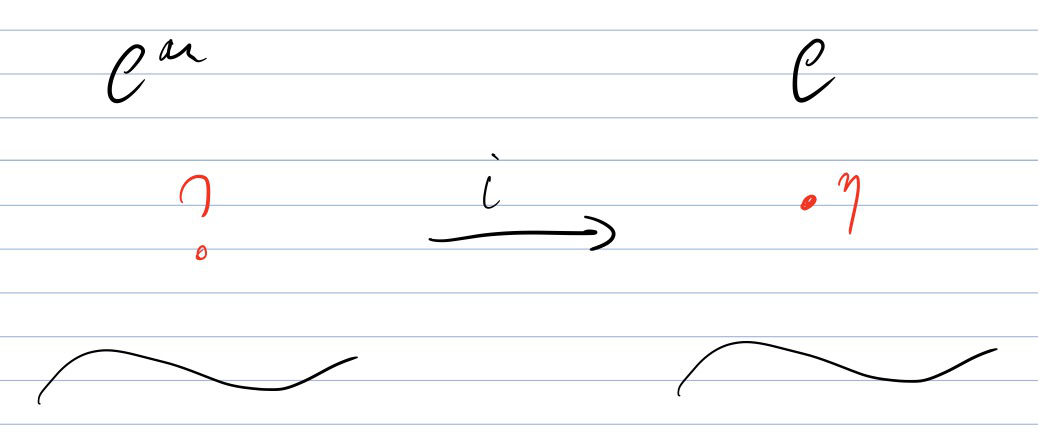
\includegraphics[width = .7\textwidth]{figures/closed-points-in-curve.png}
    \caption{closed points in curve}
    \label{fig:closed-points-in-curve}
\end{figure}

A first approach might be to take a ring and try to find all norms on that ring. 
I personally only know of two situations where a that can be done straight forwardly.
That is the affine line. 
Without going into too much detail, the affine line looks like a tree, but one where there are infinitely many branches and on every line there are infinitely many branch points. 
We will get to why this exactly is. 


\begin{definition}
	Let $C$ be a curve with snc-model $\mathcal{C} $. 
	Let $F_i$ be the irreducible components of $\mathcal{C} _s$. 
	The \emph{dual graph} is the graph with vertices $F_i$ and between every two vertices $F_i, F_j$ there are $F_i\cdot F_j$ edges. 
\end{definition}
 

\end{document}
